\documentclass[../main.tex]{subfiles}

\begin{document}
	
	
	In this section, we evaluate the performance of the trading signals generated by our particle filter when applied to EUR/USD exchange rates (For the month of Nov 2019). 
	
	Figure \ref{fig:4__3__1__trading_performance} shows the profit and loss generated by a trading strategy employing the generic RBPF with $N=1000$ particles and hyperparmeters described in \autoref{sec:experimental_hyperparameter}. The performance of the fund constructed based on the inference models developed in this project look to be very promising, with a annualized sharpe ratio of $1.10$.
	
	\begin{figure}[h!]
		\centering
		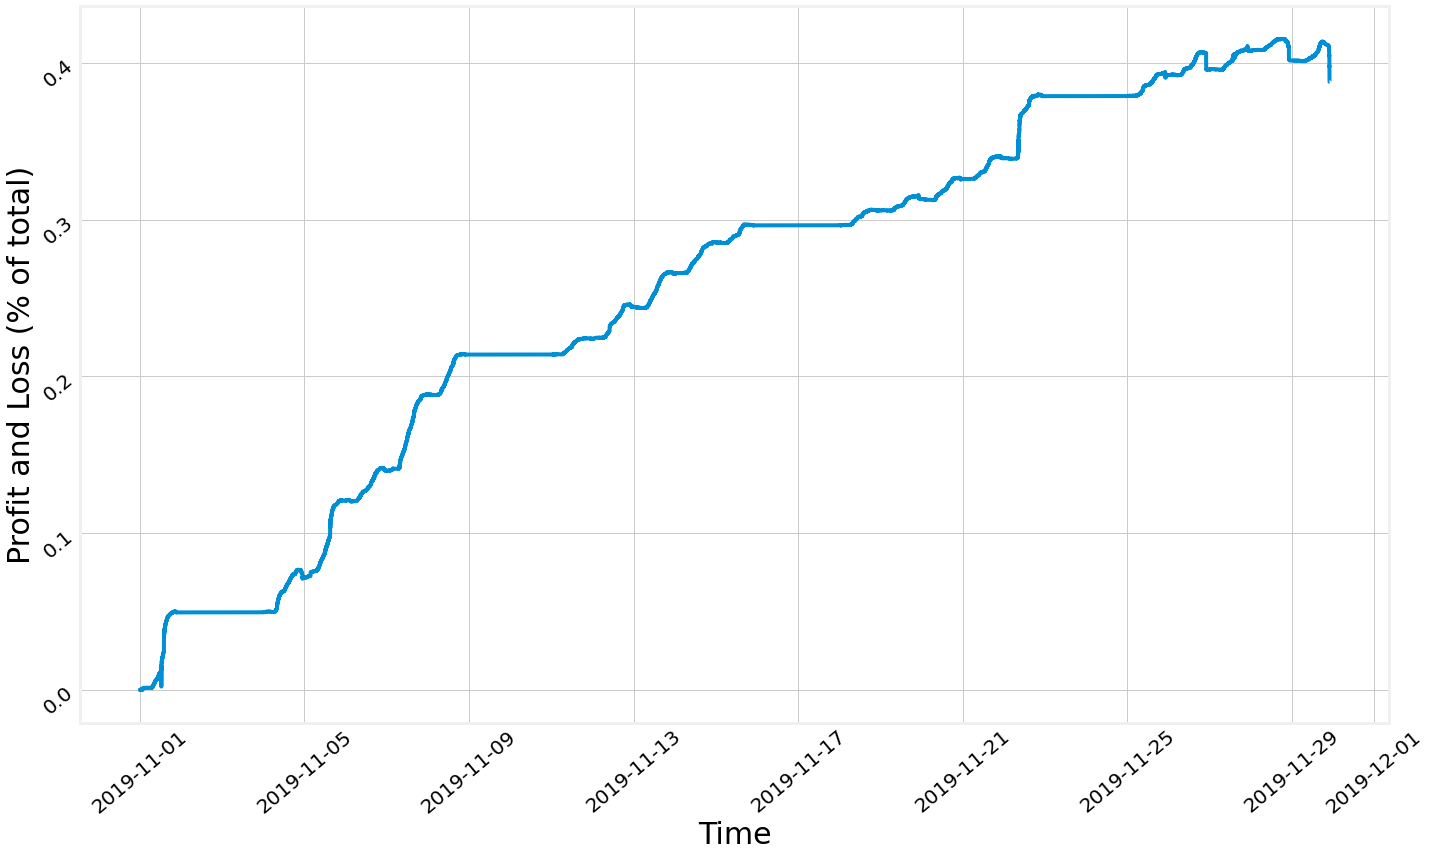
\includegraphics[width=15.0cm]{../plots/4__3__1__trading_performance.png}
		\caption{Profit and Loss (PnL) in terms of \% of the total fund}
		\label{fig:4__3__1__trading_performance}
	\end{figure}

	
\end{document}